% CC-iGPT codec dataflow figure
% Compile:  pdflatex codec_dataflow.tex
% Inline:   % CC-iGPT codec dataflow figure
% Compile:  pdflatex codec_dataflow.tex
% Inline:   % CC-iGPT codec dataflow figure
% Compile:  pdflatex codec_dataflow.tex
% Inline:   % CC-iGPT codec dataflow figure
% Compile:  pdflatex codec_dataflow.tex
% Inline:   \input{figures/codec_dataflow.tex}
%
% 配套 ctx_pipeline.tex / coarse_pipeline.tex / fine_pipeline.tex，
% 把 CC-iGPT 的「编码并行 / 解码串行」时序差异、两段式 bitstream 物理布局、
% Φ 在 enc/dec 两侧由同一函数复算（bit-exact 闭环）这三件事在一张图里讲清楚。
%
% 整体布局：
%   ┌──────────────────────────────────────────────────────────┐
%   │  [上半] Encoder：x 同时进 coarse 与 fine 两分支并行 forward │
%   │                ──► 两段算术编码 ──► 拼接                    │
%   ├──────────────────────────────────────────────────────────┤
%   │  [中央] Bitstream 盒：[coarse 64 token | fine 3072 token]  │
%   ├──────────────────────────────────────────────────────────┤
%   │  [下半] Decoder：先解 coarse → 重建 ctx → 再解 fine → 还原 │
%   │                  （串行：fine 段的解码必须等到 ctx 就绪）     │
%   └──────────────────────────────────────────────────────────┘
\documentclass[tikz,border=10pt]{standalone}
\usepackage{tikz}
\usepackage{amsmath,amssymb}
\usepackage{xcolor}
\usetikzlibrary{positioning,arrows.meta,calc,fit,backgrounds,shapes.geometric,
                decorations.pathreplacing,patterns}

\begin{document}
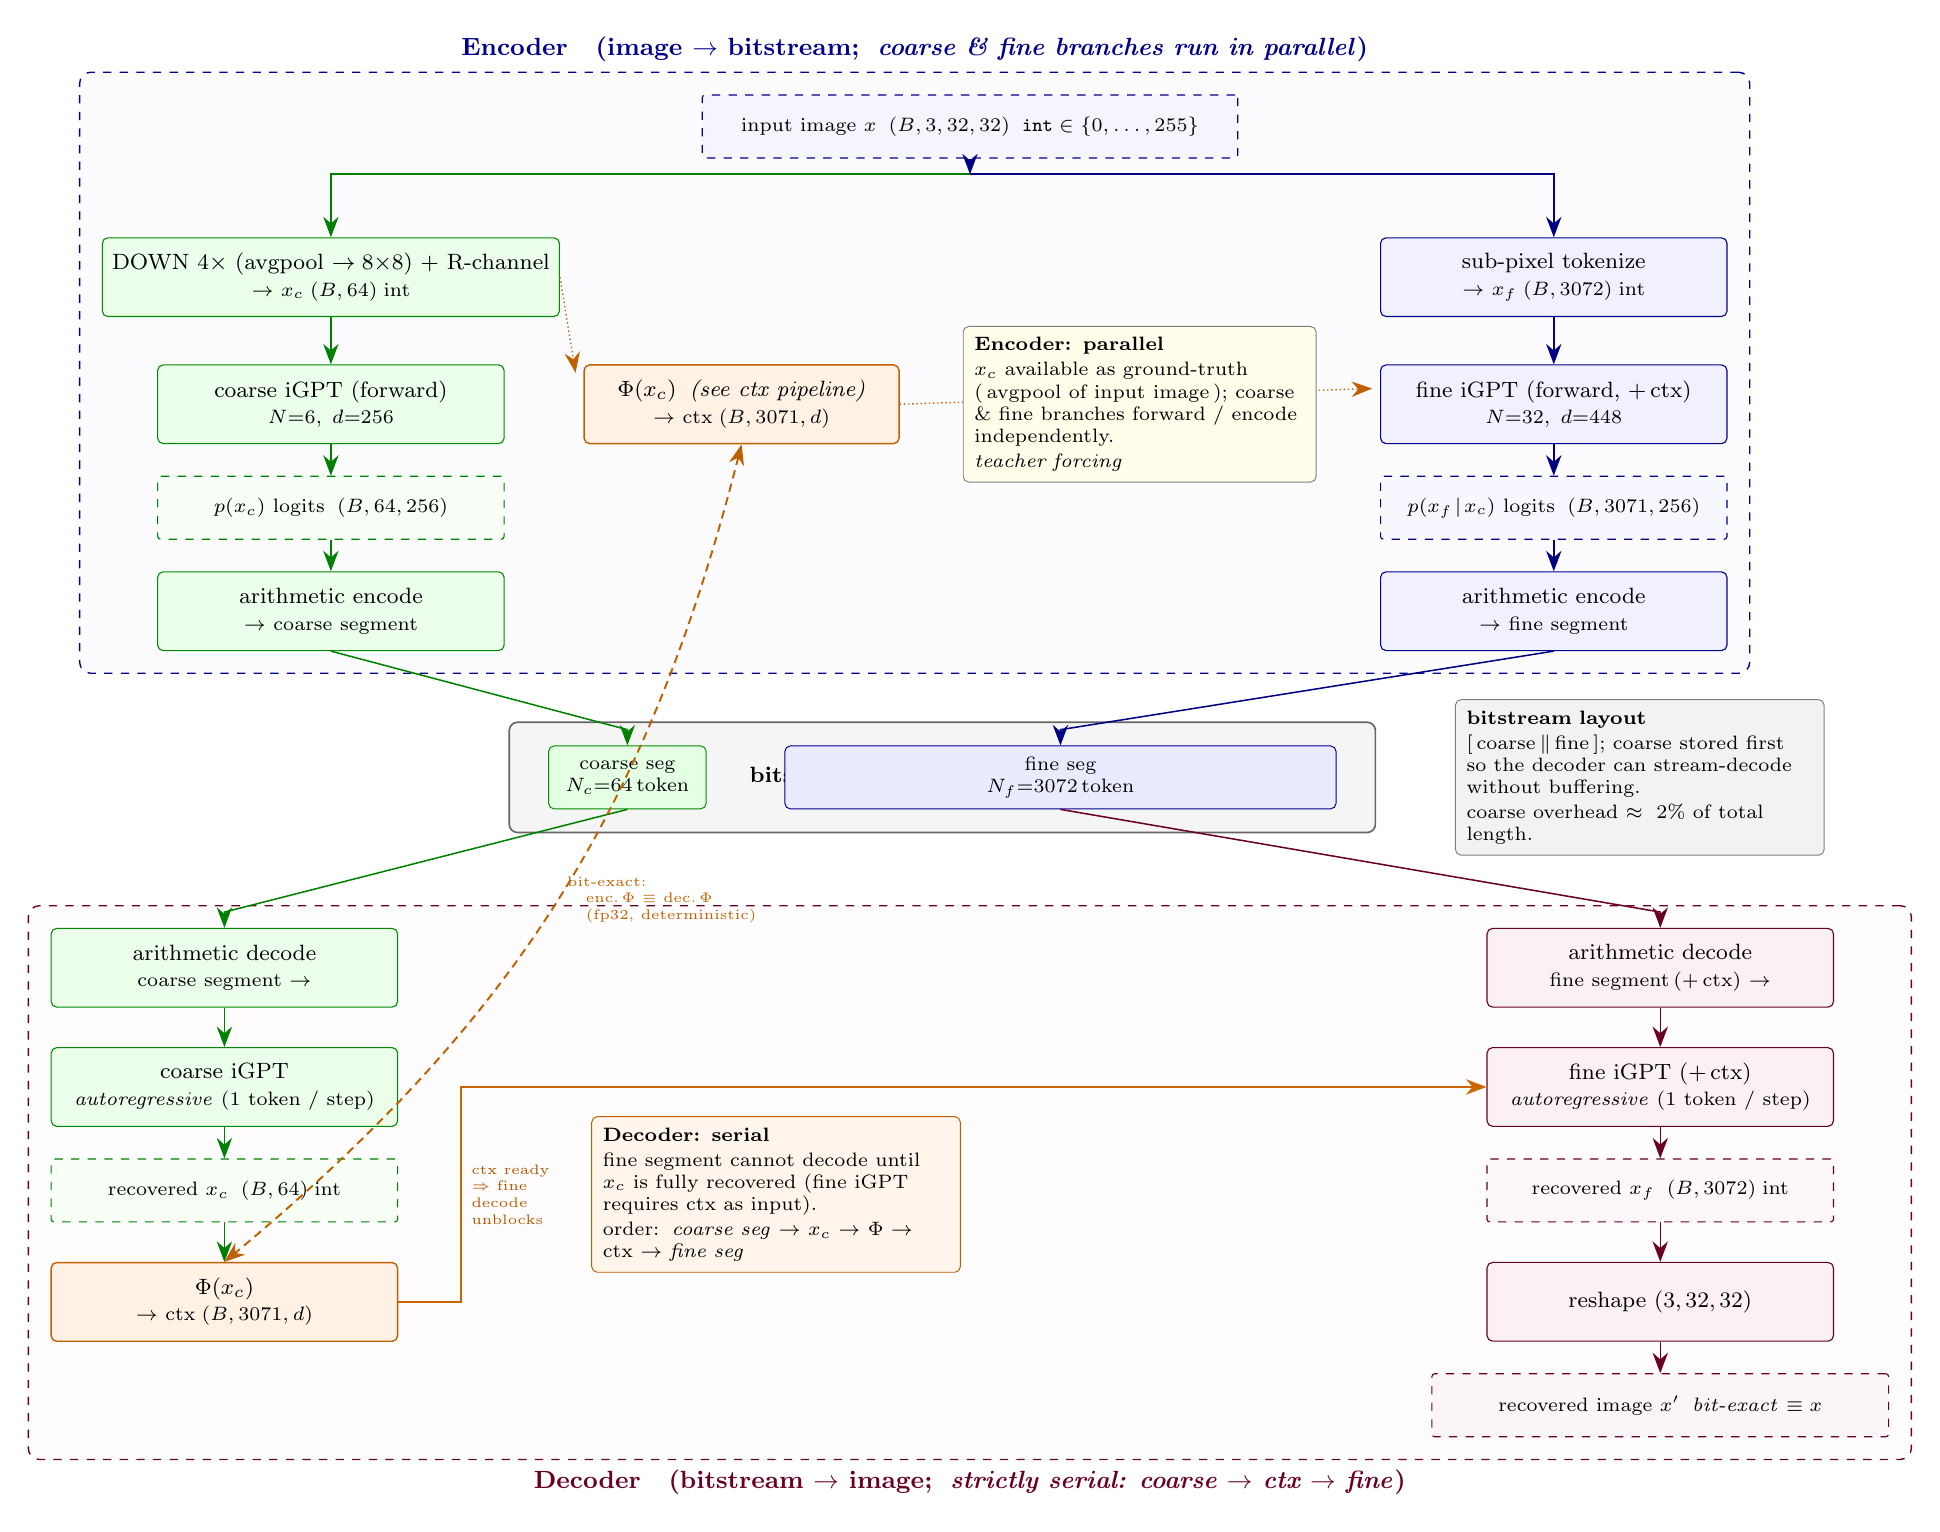
\begin{tikzpicture}[
    font=\footnotesize,
    >={Stealth[length=2.6mm]},
    node distance=8mm and 12mm,
    % ---- encoder-side blocks (top half, blue) ----
    encbox/.style ={draw, rounded corners=2pt, align=center,
                    minimum height=10mm, minimum width=44mm,
                    inner sep=3.5pt, fill=blue!6, draw=blue!55!black,
                    line width=0.4pt},
    % ---- decoder-side blocks (bottom half, purple) ----
    decbox/.style ={draw, rounded corners=2pt, align=center,
                    minimum height=10mm, minimum width=44mm,
                    inner sep=3.5pt, fill=purple!6, draw=purple!55!black,
                    line width=0.4pt},
    % ---- coarse-branch tint (green, both halves) ----
    coarsebox/.style={draw, rounded corners=2pt, align=center,
                      minimum height=10mm, minimum width=44mm,
                      inner sep=3.5pt, fill=green!8, draw=green!55!black,
                      line width=0.4pt},
    % ---- ctx box (orange, the bit-exact bridge) ----
    ctxbox/.style ={draw, rounded corners=2pt, align=center,
                    minimum height=10mm, minimum width=44mm,
                    inner sep=3.5pt, fill=orange!10, draw=orange!75!black,
                    line width=0.5pt},
    % ---- bitstream container (center, big) ----
    bsbox/.style  ={draw, rounded corners=3pt, align=center,
                    minimum height=14mm, minimum width=110mm,
                    inner sep=5pt, fill=gray!8, draw=black!60,
                    line width=0.6pt},
    bsseg/.style  ={draw, rounded corners=2pt, align=center,
                    minimum height=8mm, inner sep=3pt,
                    font=\scriptsize, line width=0.35pt},
    % ---- image / tensor pill ----
    imgpill/.style={draw, rounded corners=1pt, align=center,
                    fill=gray!4, draw=gray!55, font=\scriptsize,
                    inner sep=3pt, minimum width=44mm,
                    minimum height=8mm, dashed},
    % ---- arrows ----
    flow/.style    ={->, line width=0.55pt, blue!50!black},
    decflow/.style ={->, line width=0.55pt, purple!55!black},
    coflow/.style  ={->, line width=0.55pt, green!50!black},
    biteq/.style   ={<->, line width=0.7pt, orange!75!black, densely dashed},
    % ---- callout ----
    callout/.style ={draw=black!50, rounded corners=2pt,
                     fill=yellow!8, align=left, font=\scriptsize,
                     inner sep=4pt, line width=0.35pt},
]

% =========================================================
% TOP: encoder input (image x)
% =========================================================
\node[imgpill, fill=blue!4, draw=blue!55!black, minimum width=68mm]
     (xin) {input image $x$\;\;$(B,3,32,32)$\;\;\texttt{int}\;$\in\{0,\dots,255\}$};

% =========================================================
% Encoder split: x feeds BOTH branches in parallel
% =========================================================
% LEFT branch (coarse) and RIGHT branch (fine) at the same row
\node[coarsebox, below left=10mm and 18mm of xin]
     (e_avg) {DOWN $4{\times}$ (avgpool $\to 8{\times}8$) + R-channel\\\scriptsize $\to$ $x_c$\;$(B,64)$\;int};
\node[encbox, below right=10mm and 18mm of xin]
     (e_tok) {sub-pixel tokenize\\\scriptsize $\to$ $x_f$\;$(B,3072)$\;int};

% Coarse encoder chain
\node[coarsebox, below=6mm of e_avg] (e_cgpt)
     {coarse iGPT (forward)\\\scriptsize $N{=}6,\;d{=}256$};
\node[imgpill, below=4mm of e_cgpt, fill=green!3, draw=green!50!black]
     (e_cprob) {$p(x_c)$ logits\;\;$(B,64,256)$};
\node[coarsebox, below=4mm of e_cprob] (e_cac)
     {arithmetic encode\\\scriptsize $\to$ coarse segment};

% Fine encoder chain
\node[encbox, below=6mm of e_tok] (e_fgpt)
     {fine iGPT (forward, +\,ctx)\\\scriptsize $N{=}32,\;d{=}448$};
\node[imgpill, below=4mm of e_fgpt, fill=blue!3, draw=blue!50!black]
     (e_fprob) {$p(x_f\!\mid\! x_c)$ logits\;\;$(B,3071,256)$};
\node[encbox, below=4mm of e_fprob] (e_fac)
     {arithmetic encode\\\scriptsize $\to$ fine segment};

% Encoder-side ctx (between the two chains, fed to fine)
\node[ctxbox, right=10mm of e_cgpt, minimum width=40mm]
     (e_phi) {$\Phi(x_c)$\;\;\textit{(see ctx pipeline)}\\\scriptsize $\to$ ctx\;$(B,3071,d)$};

% =========================================================
% Center: bitstream box (the meeting point)
% =========================================================
\node[bsbox, below=14mm of $(e_cac)!0.5!(e_fac)$] (bs)
     {\textbf{bitstream} \;(persistent / wire / disk)};
\node[bsseg, fill=green!10, draw=green!55!black, minimum width=20mm]
     at ($(bs.center)+(-40mm,0)$)
     (bsCo) {coarse seg\\$N_c{=}64$\,token};
\node[bsseg, fill=blue!8, draw=blue!55!black, minimum width=70mm]
     at ($(bs.center)+(15mm,0)$)
     (bsFi) {fine seg\\$N_f{=}3072$\,token};

% =========================================================
% BOTTOM: decoder chain (strictly serial)
% =========================================================
% Decoder coarse branch (LEFT, mirrors encoder)
\node[coarsebox, below left=12mm and 14mm of bs] (d_cac)
     {arithmetic decode\\\scriptsize coarse segment $\to$};
\node[coarsebox, below=5mm of d_cac] (d_cgpt)
     {coarse iGPT\\\scriptsize \emph{autoregressive} (1 token / step)};
\node[imgpill, below=4mm of d_cgpt, fill=green!3, draw=green!50!black]
     (d_xc) {recovered $x_c$\;\;$(B,64)$\;int};
\node[ctxbox, below=5mm of d_xc, minimum width=44mm]
     (d_phi) {$\Phi(x_c)$\\\scriptsize $\to$ ctx\;$(B,3071,d)$};

% Decoder fine branch (RIGHT, depends on ctx)
\node[decbox, below right=12mm and 14mm of bs] (d_fac)
     {arithmetic decode\\\scriptsize fine segment\,(+\,ctx) $\to$};
\node[decbox, below=5mm of d_fac] (d_fgpt)
     {fine iGPT (+\,ctx)\\\scriptsize \emph{autoregressive} (1 token / step)};
\node[imgpill, below=4mm of d_fgpt, fill=purple!3, draw=purple!50!black]
     (d_xf) {recovered $x_f$\;\;$(B,3072)$\;int};
\node[decbox, below=5mm of d_xf] (d_reshape)
     {reshape $(3,32,32)$};
\node[imgpill, below=4mm of d_reshape, fill=purple!4, draw=purple!55!black,
      minimum width=58mm]
     (xout) {recovered image $x'$\;\;\textit{bit-exact} $\equiv x$};

% =========================================================
% Encoder arrows
% =========================================================
\draw[flow] (xin.south) -- ++(0,-2mm) coordinate (xsplit);
\draw[coflow] (xsplit) -| (e_avg.north);
\draw[flow]   (xsplit) -| (e_tok.north);

\draw[coflow] (e_avg) -- (e_cgpt);
\draw[coflow] (e_cgpt) -- (e_cprob);
\draw[coflow] (e_cprob) -- (e_cac);

\draw[flow] (e_tok) -- (e_fgpt);
\draw[flow] (e_fgpt) -- (e_fprob);
\draw[flow] (e_fprob) -- (e_fac);

% encoder ctx feed: x_c (avg/coarse output) -> Phi -> fine iGPT
\draw[->, line width=0.5pt, orange!75!black, densely dotted]
     (e_avg.east) -- ($(e_phi.west)+(-1mm,4mm)$);
\draw[->, line width=0.5pt, orange!75!black, densely dotted]
     (e_phi.east) -- ($(e_fgpt.west)+(-1mm,2mm)$)
     node[midway, above, font=\tiny, orange!60!black]
     {$\alpha\!\cdot\!$ctx};

% encoder -> bitstream
\draw[coflow] (e_cac.south) -- ($(bsCo.north)+(0,2mm)$) -- (bsCo.north);
\draw[flow]   (e_fac.south) -- ($(bsFi.north)+(0,2mm)$) -- (bsFi.north);

% =========================================================
% Decoder arrows
% =========================================================
% bitstream -> decoder
\draw[coflow] (bsCo.south) -- ($(d_cac.north)+(0,2mm)$) -- (d_cac.north);
\draw[decflow] (bsFi.south) -- ($(d_fac.north)+(0,2mm)$) -- (d_fac.north);

% decoder coarse chain
\draw[coflow] (d_cac) -- (d_cgpt);
\draw[coflow] (d_cgpt) -- (d_xc);
\draw[coflow] (d_xc) -- (d_phi);

% the critical cross-coupling: Phi -> fine decoder (serial dependency)
\draw[->, line width=0.7pt, orange!80!black]
     (d_phi.east) -- ++(8mm,0) |- (d_fgpt.west)
     node[pos=0.25, right, font=\tiny, orange!70!black, align=left,
          name=unblockLbl]
     {ctx ready\\$\Rightarrow$ fine\\decode\\unblocks};

% decoder fine chain
\draw[decflow] (d_fac) -- (d_fgpt);
\draw[decflow] (d_fgpt) -- (d_xf);
\draw[decflow] (d_xf) -- (d_reshape);
\draw[decflow] (d_reshape) -- (xout);

% =========================================================
% bit-exact equivalence (Phi enc == Phi dec) -- the central guarantee
% =========================================================
\draw[biteq] (e_phi.south) to[bend left=18]
             node[midway, right, font=\tiny, orange!75!black, align=left]
             {bit-exact:\\\quad enc.\,$\Phi$ $\equiv$ dec.\,$\Phi$\\\quad (fp32, deterministic)}
             (d_phi.north);

% =========================================================
% Section frames + labels
% =========================================================
\begin{pgfonlayer}{background}
  % Encoder frame (top half)
  \node[draw=blue!55!black, dashed, rounded corners=4pt,
        fill=blue!1, line width=0.5pt, inner sep=8pt,
        fit=(xin)(e_avg)(e_tok)(e_cgpt)(e_fgpt)(e_phi)(e_cac)(e_fac),
        label={[blue!55!black, font=\small\bfseries]above:%
              \textbf{Encoder} \; (image $\to$ bitstream;\;
              \emph{coarse \& fine branches run in parallel})}]
        (encframe) {};

  % Decoder frame (bottom half)
  \node[draw=purple!55!black, dashed, rounded corners=4pt,
        fill=purple!1, line width=0.5pt, inner sep=8pt,
        fit=(d_cac)(d_fac)(d_cgpt)(d_fgpt)(d_xc)(d_phi)(d_xf)(d_reshape)(xout),
        label={[purple!55!black, font=\small\bfseries]below:%
              \textbf{Decoder} \; (bitstream $\to$ image;\;
              \emph{strictly serial: coarse $\to$ ctx $\to$ fine})}]
        (decframe) {};
\end{pgfonlayer}

% =========================================================
% Right-side legend / callouts
% =========================================================
\node[callout, right=8mm of e_phi, text width=42mm, anchor=west]
     (legA) {\textbf{Encoder: parallel}\\[1pt]
             $x_c$ available as ground-truth (\,avgpool of input image\,);
             coarse \& fine branches forward / encode independently.\\[1pt]
             \textit{teacher forcing}};

\node[callout, right=4mm of unblockLbl, anchor=west, text width=44mm,
      fill=orange!8, draw=orange!75!black]
     (legB) {\textbf{Decoder: serial}\\[1pt]
             fine segment cannot decode until $x_c$ is fully recovered
             (fine iGPT requires ctx as input).\\[1pt]
             order:\;\;\emph{coarse seg} $\to$ $x_c$ $\to$ $\Phi$ $\to$ ctx
             $\to$ \emph{fine seg}};

\node[callout, right=10mm of bs, text width=44mm, anchor=west,
      fill=gray!10, draw=black!50]
     (legBS){\textbf{bitstream layout}\\[1pt]
             $[\,\text{coarse}\,\Vert\,\text{fine}\,]$;
             coarse stored first so the decoder can stream-decode
             without buffering.\\[1pt]
             coarse overhead $\approx 2\%$ of total length.};

\end{tikzpicture}
\end{document}

%
% 配套 ctx_pipeline.tex / coarse_pipeline.tex / fine_pipeline.tex，
% 把 CC-iGPT 的「编码并行 / 解码串行」时序差异、两段式 bitstream 物理布局、
% Φ 在 enc/dec 两侧由同一函数复算（bit-exact 闭环）这三件事在一张图里讲清楚。
%
% 整体布局：
%   ┌──────────────────────────────────────────────────────────┐
%   │  [上半] Encoder：x 同时进 coarse 与 fine 两分支并行 forward │
%   │                ──► 两段算术编码 ──► 拼接                    │
%   ├──────────────────────────────────────────────────────────┤
%   │  [中央] Bitstream 盒：[coarse 64 token | fine 3072 token]  │
%   ├──────────────────────────────────────────────────────────┤
%   │  [下半] Decoder：先解 coarse → 重建 ctx → 再解 fine → 还原 │
%   │                  （串行：fine 段的解码必须等到 ctx 就绪）     │
%   └──────────────────────────────────────────────────────────┘
\documentclass[tikz,border=10pt]{standalone}
\usepackage{tikz}
\usepackage{amsmath,amssymb}
\usepackage{xcolor}
\usetikzlibrary{positioning,arrows.meta,calc,fit,backgrounds,shapes.geometric,
                decorations.pathreplacing,patterns}

\begin{document}
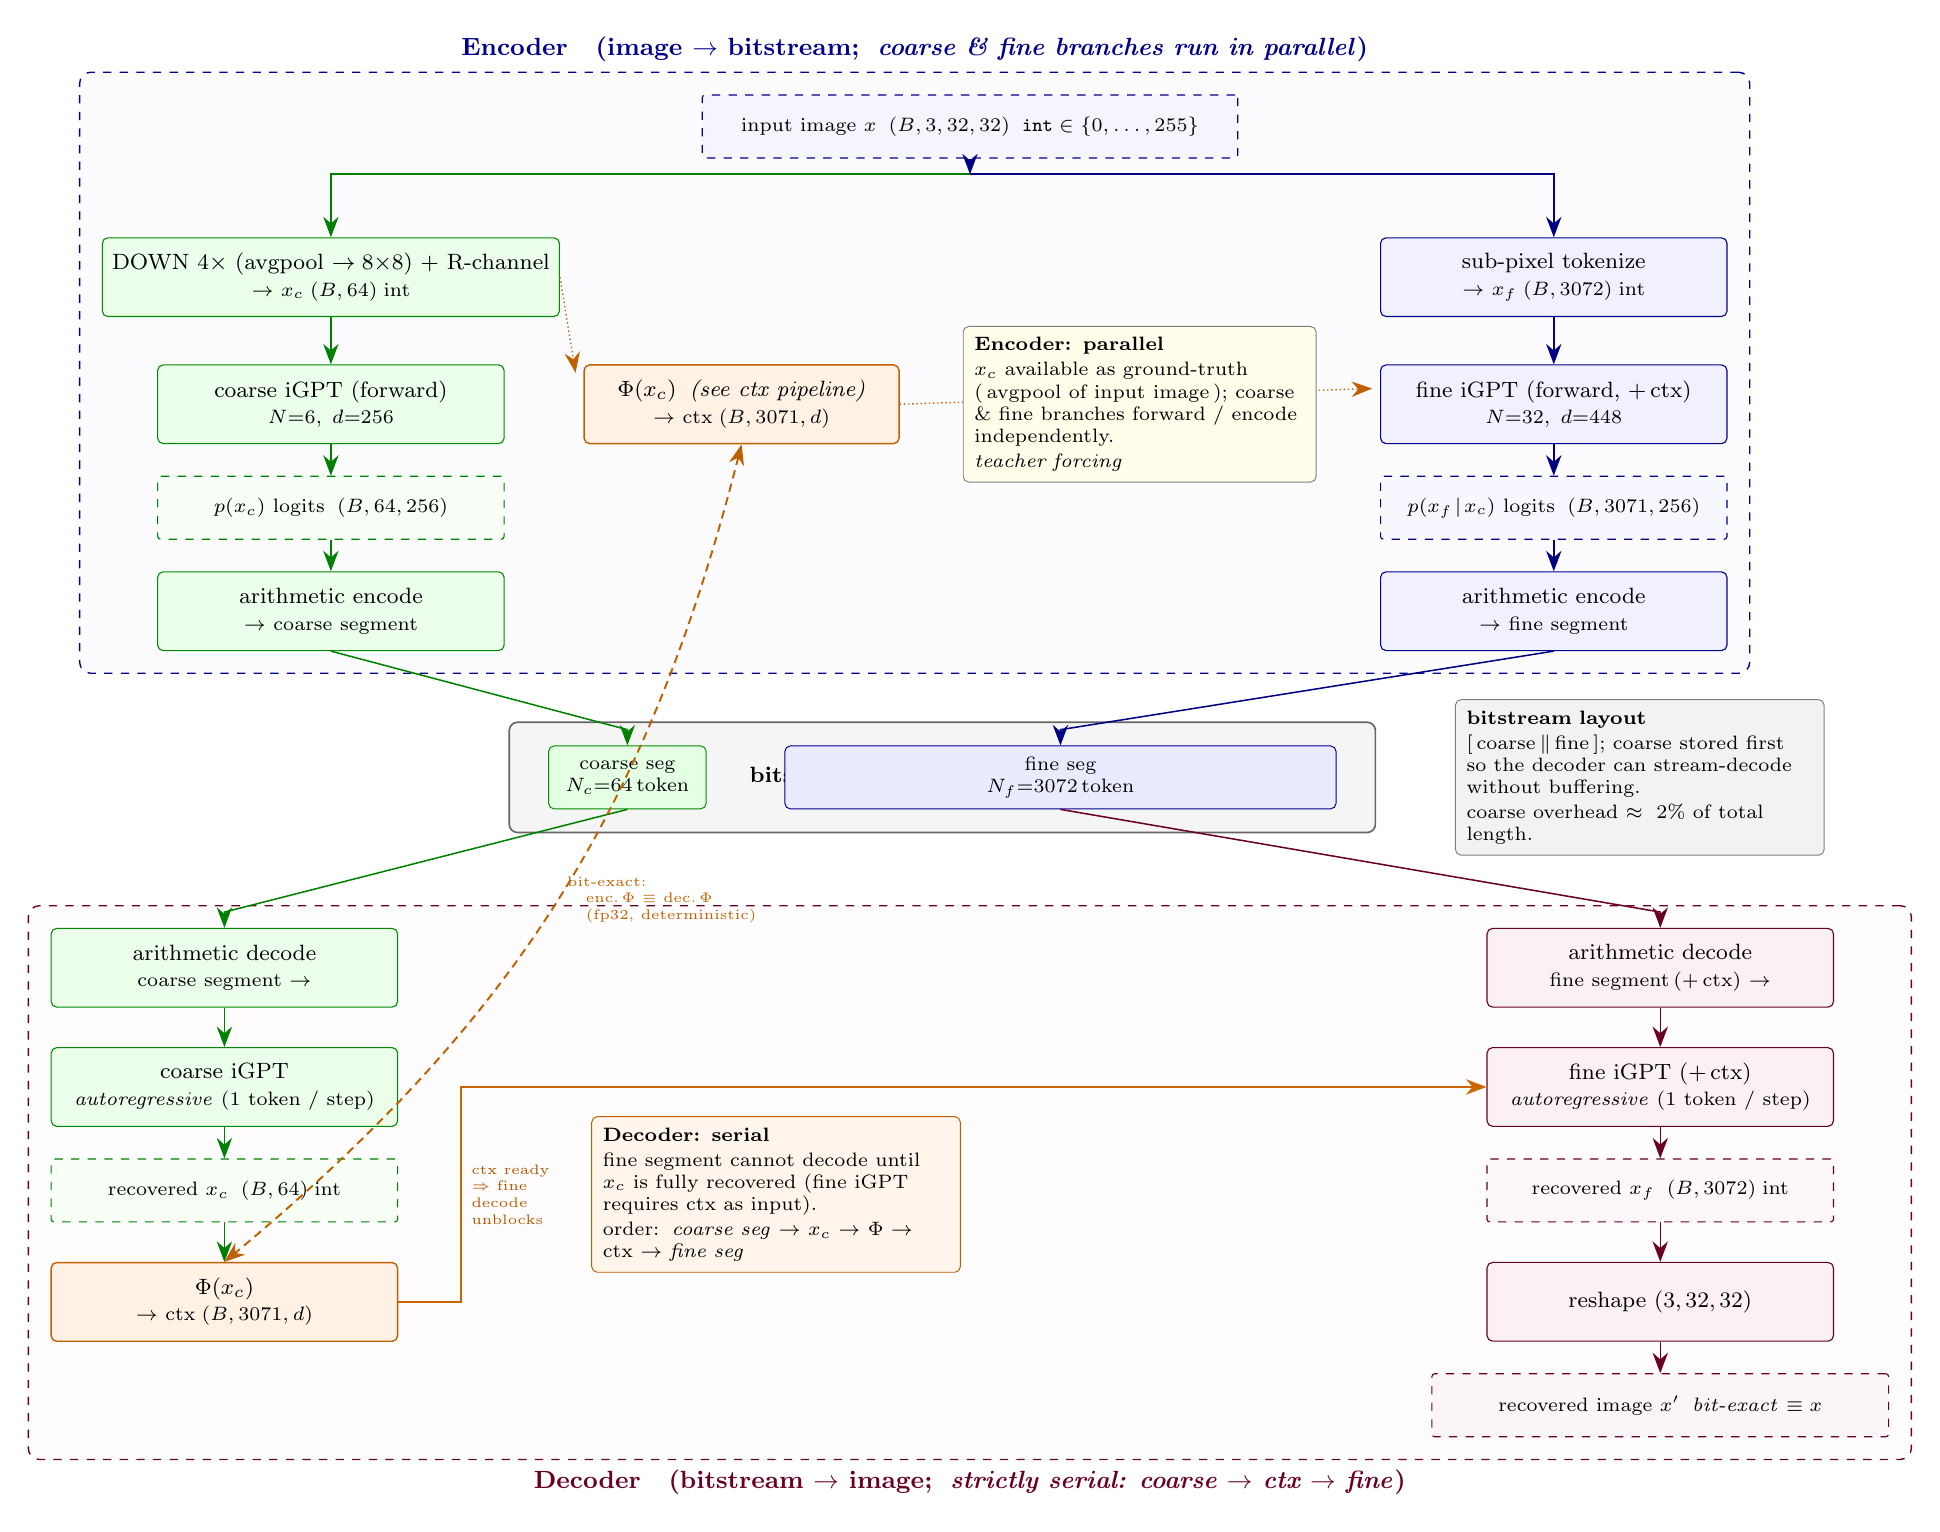
\begin{tikzpicture}[
    font=\footnotesize,
    >={Stealth[length=2.6mm]},
    node distance=8mm and 12mm,
    % ---- encoder-side blocks (top half, blue) ----
    encbox/.style ={draw, rounded corners=2pt, align=center,
                    minimum height=10mm, minimum width=44mm,
                    inner sep=3.5pt, fill=blue!6, draw=blue!55!black,
                    line width=0.4pt},
    % ---- decoder-side blocks (bottom half, purple) ----
    decbox/.style ={draw, rounded corners=2pt, align=center,
                    minimum height=10mm, minimum width=44mm,
                    inner sep=3.5pt, fill=purple!6, draw=purple!55!black,
                    line width=0.4pt},
    % ---- coarse-branch tint (green, both halves) ----
    coarsebox/.style={draw, rounded corners=2pt, align=center,
                      minimum height=10mm, minimum width=44mm,
                      inner sep=3.5pt, fill=green!8, draw=green!55!black,
                      line width=0.4pt},
    % ---- ctx box (orange, the bit-exact bridge) ----
    ctxbox/.style ={draw, rounded corners=2pt, align=center,
                    minimum height=10mm, minimum width=44mm,
                    inner sep=3.5pt, fill=orange!10, draw=orange!75!black,
                    line width=0.5pt},
    % ---- bitstream container (center, big) ----
    bsbox/.style  ={draw, rounded corners=3pt, align=center,
                    minimum height=14mm, minimum width=110mm,
                    inner sep=5pt, fill=gray!8, draw=black!60,
                    line width=0.6pt},
    bsseg/.style  ={draw, rounded corners=2pt, align=center,
                    minimum height=8mm, inner sep=3pt,
                    font=\scriptsize, line width=0.35pt},
    % ---- image / tensor pill ----
    imgpill/.style={draw, rounded corners=1pt, align=center,
                    fill=gray!4, draw=gray!55, font=\scriptsize,
                    inner sep=3pt, minimum width=44mm,
                    minimum height=8mm, dashed},
    % ---- arrows ----
    flow/.style    ={->, line width=0.55pt, blue!50!black},
    decflow/.style ={->, line width=0.55pt, purple!55!black},
    coflow/.style  ={->, line width=0.55pt, green!50!black},
    biteq/.style   ={<->, line width=0.7pt, orange!75!black, densely dashed},
    % ---- callout ----
    callout/.style ={draw=black!50, rounded corners=2pt,
                     fill=yellow!8, align=left, font=\scriptsize,
                     inner sep=4pt, line width=0.35pt},
]

% =========================================================
% TOP: encoder input (image x)
% =========================================================
\node[imgpill, fill=blue!4, draw=blue!55!black, minimum width=68mm]
     (xin) {input image $x$\;\;$(B,3,32,32)$\;\;\texttt{int}\;$\in\{0,\dots,255\}$};

% =========================================================
% Encoder split: x feeds BOTH branches in parallel
% =========================================================
% LEFT branch (coarse) and RIGHT branch (fine) at the same row
\node[coarsebox, below left=10mm and 18mm of xin]
     (e_avg) {DOWN $4{\times}$ (avgpool $\to 8{\times}8$) + R-channel\\\scriptsize $\to$ $x_c$\;$(B,64)$\;int};
\node[encbox, below right=10mm and 18mm of xin]
     (e_tok) {sub-pixel tokenize\\\scriptsize $\to$ $x_f$\;$(B,3072)$\;int};

% Coarse encoder chain
\node[coarsebox, below=6mm of e_avg] (e_cgpt)
     {coarse iGPT (forward)\\\scriptsize $N{=}6,\;d{=}256$};
\node[imgpill, below=4mm of e_cgpt, fill=green!3, draw=green!50!black]
     (e_cprob) {$p(x_c)$ logits\;\;$(B,64,256)$};
\node[coarsebox, below=4mm of e_cprob] (e_cac)
     {arithmetic encode\\\scriptsize $\to$ coarse segment};

% Fine encoder chain
\node[encbox, below=6mm of e_tok] (e_fgpt)
     {fine iGPT (forward, +\,ctx)\\\scriptsize $N{=}32,\;d{=}448$};
\node[imgpill, below=4mm of e_fgpt, fill=blue!3, draw=blue!50!black]
     (e_fprob) {$p(x_f\!\mid\! x_c)$ logits\;\;$(B,3071,256)$};
\node[encbox, below=4mm of e_fprob] (e_fac)
     {arithmetic encode\\\scriptsize $\to$ fine segment};

% Encoder-side ctx (between the two chains, fed to fine)
\node[ctxbox, right=10mm of e_cgpt, minimum width=40mm]
     (e_phi) {$\Phi(x_c)$\;\;\textit{(see ctx pipeline)}\\\scriptsize $\to$ ctx\;$(B,3071,d)$};

% =========================================================
% Center: bitstream box (the meeting point)
% =========================================================
\node[bsbox, below=14mm of $(e_cac)!0.5!(e_fac)$] (bs)
     {\textbf{bitstream} \;(persistent / wire / disk)};
\node[bsseg, fill=green!10, draw=green!55!black, minimum width=20mm]
     at ($(bs.center)+(-40mm,0)$)
     (bsCo) {coarse seg\\$N_c{=}64$\,token};
\node[bsseg, fill=blue!8, draw=blue!55!black, minimum width=70mm]
     at ($(bs.center)+(15mm,0)$)
     (bsFi) {fine seg\\$N_f{=}3072$\,token};

% =========================================================
% BOTTOM: decoder chain (strictly serial)
% =========================================================
% Decoder coarse branch (LEFT, mirrors encoder)
\node[coarsebox, below left=12mm and 14mm of bs] (d_cac)
     {arithmetic decode\\\scriptsize coarse segment $\to$};
\node[coarsebox, below=5mm of d_cac] (d_cgpt)
     {coarse iGPT\\\scriptsize \emph{autoregressive} (1 token / step)};
\node[imgpill, below=4mm of d_cgpt, fill=green!3, draw=green!50!black]
     (d_xc) {recovered $x_c$\;\;$(B,64)$\;int};
\node[ctxbox, below=5mm of d_xc, minimum width=44mm]
     (d_phi) {$\Phi(x_c)$\\\scriptsize $\to$ ctx\;$(B,3071,d)$};

% Decoder fine branch (RIGHT, depends on ctx)
\node[decbox, below right=12mm and 14mm of bs] (d_fac)
     {arithmetic decode\\\scriptsize fine segment\,(+\,ctx) $\to$};
\node[decbox, below=5mm of d_fac] (d_fgpt)
     {fine iGPT (+\,ctx)\\\scriptsize \emph{autoregressive} (1 token / step)};
\node[imgpill, below=4mm of d_fgpt, fill=purple!3, draw=purple!50!black]
     (d_xf) {recovered $x_f$\;\;$(B,3072)$\;int};
\node[decbox, below=5mm of d_xf] (d_reshape)
     {reshape $(3,32,32)$};
\node[imgpill, below=4mm of d_reshape, fill=purple!4, draw=purple!55!black,
      minimum width=58mm]
     (xout) {recovered image $x'$\;\;\textit{bit-exact} $\equiv x$};

% =========================================================
% Encoder arrows
% =========================================================
\draw[flow] (xin.south) -- ++(0,-2mm) coordinate (xsplit);
\draw[coflow] (xsplit) -| (e_avg.north);
\draw[flow]   (xsplit) -| (e_tok.north);

\draw[coflow] (e_avg) -- (e_cgpt);
\draw[coflow] (e_cgpt) -- (e_cprob);
\draw[coflow] (e_cprob) -- (e_cac);

\draw[flow] (e_tok) -- (e_fgpt);
\draw[flow] (e_fgpt) -- (e_fprob);
\draw[flow] (e_fprob) -- (e_fac);

% encoder ctx feed: x_c (avg/coarse output) -> Phi -> fine iGPT
\draw[->, line width=0.5pt, orange!75!black, densely dotted]
     (e_avg.east) -- ($(e_phi.west)+(-1mm,4mm)$);
\draw[->, line width=0.5pt, orange!75!black, densely dotted]
     (e_phi.east) -- ($(e_fgpt.west)+(-1mm,2mm)$)
     node[midway, above, font=\tiny, orange!60!black]
     {$\alpha\!\cdot\!$ctx};

% encoder -> bitstream
\draw[coflow] (e_cac.south) -- ($(bsCo.north)+(0,2mm)$) -- (bsCo.north);
\draw[flow]   (e_fac.south) -- ($(bsFi.north)+(0,2mm)$) -- (bsFi.north);

% =========================================================
% Decoder arrows
% =========================================================
% bitstream -> decoder
\draw[coflow] (bsCo.south) -- ($(d_cac.north)+(0,2mm)$) -- (d_cac.north);
\draw[decflow] (bsFi.south) -- ($(d_fac.north)+(0,2mm)$) -- (d_fac.north);

% decoder coarse chain
\draw[coflow] (d_cac) -- (d_cgpt);
\draw[coflow] (d_cgpt) -- (d_xc);
\draw[coflow] (d_xc) -- (d_phi);

% the critical cross-coupling: Phi -> fine decoder (serial dependency)
\draw[->, line width=0.7pt, orange!80!black]
     (d_phi.east) -- ++(8mm,0) |- (d_fgpt.west)
     node[pos=0.25, right, font=\tiny, orange!70!black, align=left,
          name=unblockLbl]
     {ctx ready\\$\Rightarrow$ fine\\decode\\unblocks};

% decoder fine chain
\draw[decflow] (d_fac) -- (d_fgpt);
\draw[decflow] (d_fgpt) -- (d_xf);
\draw[decflow] (d_xf) -- (d_reshape);
\draw[decflow] (d_reshape) -- (xout);

% =========================================================
% bit-exact equivalence (Phi enc == Phi dec) -- the central guarantee
% =========================================================
\draw[biteq] (e_phi.south) to[bend left=18]
             node[midway, right, font=\tiny, orange!75!black, align=left]
             {bit-exact:\\\quad enc.\,$\Phi$ $\equiv$ dec.\,$\Phi$\\\quad (fp32, deterministic)}
             (d_phi.north);

% =========================================================
% Section frames + labels
% =========================================================
\begin{pgfonlayer}{background}
  % Encoder frame (top half)
  \node[draw=blue!55!black, dashed, rounded corners=4pt,
        fill=blue!1, line width=0.5pt, inner sep=8pt,
        fit=(xin)(e_avg)(e_tok)(e_cgpt)(e_fgpt)(e_phi)(e_cac)(e_fac),
        label={[blue!55!black, font=\small\bfseries]above:%
              \textbf{Encoder} \; (image $\to$ bitstream;\;
              \emph{coarse \& fine branches run in parallel})}]
        (encframe) {};

  % Decoder frame (bottom half)
  \node[draw=purple!55!black, dashed, rounded corners=4pt,
        fill=purple!1, line width=0.5pt, inner sep=8pt,
        fit=(d_cac)(d_fac)(d_cgpt)(d_fgpt)(d_xc)(d_phi)(d_xf)(d_reshape)(xout),
        label={[purple!55!black, font=\small\bfseries]below:%
              \textbf{Decoder} \; (bitstream $\to$ image;\;
              \emph{strictly serial: coarse $\to$ ctx $\to$ fine})}]
        (decframe) {};
\end{pgfonlayer}

% =========================================================
% Right-side legend / callouts
% =========================================================
\node[callout, right=8mm of e_phi, text width=42mm, anchor=west]
     (legA) {\textbf{Encoder: parallel}\\[1pt]
             $x_c$ available as ground-truth (\,avgpool of input image\,);
             coarse \& fine branches forward / encode independently.\\[1pt]
             \textit{teacher forcing}};

\node[callout, right=4mm of unblockLbl, anchor=west, text width=44mm,
      fill=orange!8, draw=orange!75!black]
     (legB) {\textbf{Decoder: serial}\\[1pt]
             fine segment cannot decode until $x_c$ is fully recovered
             (fine iGPT requires ctx as input).\\[1pt]
             order:\;\;\emph{coarse seg} $\to$ $x_c$ $\to$ $\Phi$ $\to$ ctx
             $\to$ \emph{fine seg}};

\node[callout, right=10mm of bs, text width=44mm, anchor=west,
      fill=gray!10, draw=black!50]
     (legBS){\textbf{bitstream layout}\\[1pt]
             $[\,\text{coarse}\,\Vert\,\text{fine}\,]$;
             coarse stored first so the decoder can stream-decode
             without buffering.\\[1pt]
             coarse overhead $\approx 2\%$ of total length.};

\end{tikzpicture}
\end{document}

%
% 配套 ctx_pipeline.tex / coarse_pipeline.tex / fine_pipeline.tex，
% 把 CC-iGPT 的「编码并行 / 解码串行」时序差异、两段式 bitstream 物理布局、
% Φ 在 enc/dec 两侧由同一函数复算（bit-exact 闭环）这三件事在一张图里讲清楚。
%
% 整体布局：
%   ┌──────────────────────────────────────────────────────────┐
%   │  [上半] Encoder：x 同时进 coarse 与 fine 两分支并行 forward │
%   │                ──► 两段算术编码 ──► 拼接                    │
%   ├──────────────────────────────────────────────────────────┤
%   │  [中央] Bitstream 盒：[coarse 64 token | fine 3072 token]  │
%   ├──────────────────────────────────────────────────────────┤
%   │  [下半] Decoder：先解 coarse → 重建 ctx → 再解 fine → 还原 │
%   │                  （串行：fine 段的解码必须等到 ctx 就绪）     │
%   └──────────────────────────────────────────────────────────┘
\documentclass[tikz,border=10pt]{standalone}
\usepackage{tikz}
\usepackage{amsmath,amssymb}
\usepackage{xcolor}
\usetikzlibrary{positioning,arrows.meta,calc,fit,backgrounds,shapes.geometric,
                decorations.pathreplacing,patterns}

\begin{document}
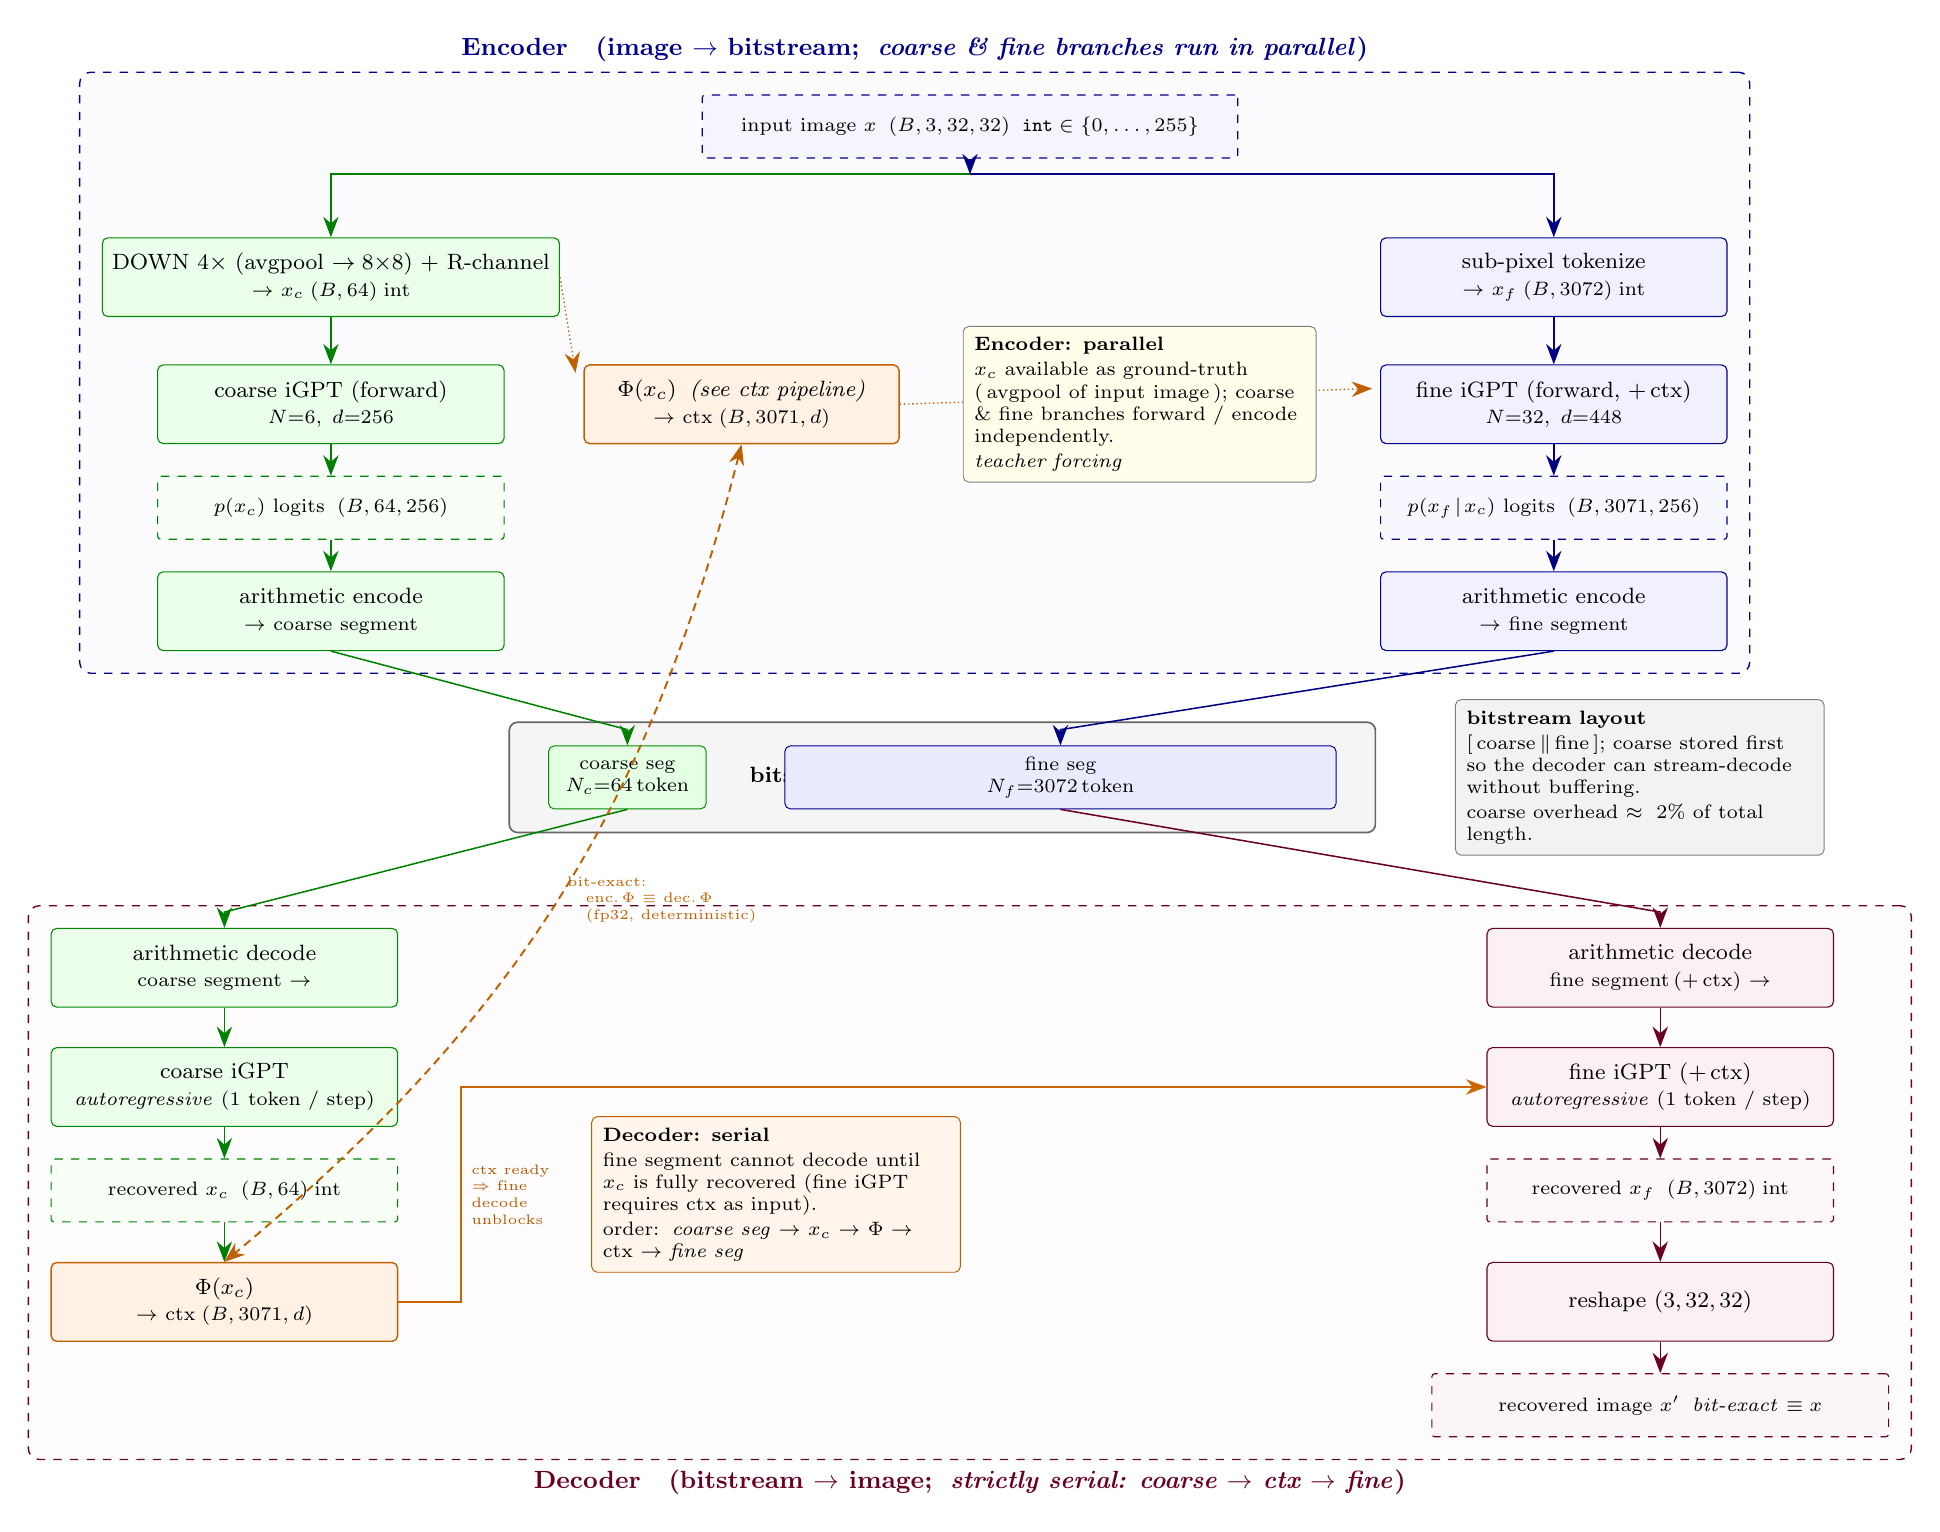
\begin{tikzpicture}[
    font=\footnotesize,
    >={Stealth[length=2.6mm]},
    node distance=8mm and 12mm,
    % ---- encoder-side blocks (top half, blue) ----
    encbox/.style ={draw, rounded corners=2pt, align=center,
                    minimum height=10mm, minimum width=44mm,
                    inner sep=3.5pt, fill=blue!6, draw=blue!55!black,
                    line width=0.4pt},
    % ---- decoder-side blocks (bottom half, purple) ----
    decbox/.style ={draw, rounded corners=2pt, align=center,
                    minimum height=10mm, minimum width=44mm,
                    inner sep=3.5pt, fill=purple!6, draw=purple!55!black,
                    line width=0.4pt},
    % ---- coarse-branch tint (green, both halves) ----
    coarsebox/.style={draw, rounded corners=2pt, align=center,
                      minimum height=10mm, minimum width=44mm,
                      inner sep=3.5pt, fill=green!8, draw=green!55!black,
                      line width=0.4pt},
    % ---- ctx box (orange, the bit-exact bridge) ----
    ctxbox/.style ={draw, rounded corners=2pt, align=center,
                    minimum height=10mm, minimum width=44mm,
                    inner sep=3.5pt, fill=orange!10, draw=orange!75!black,
                    line width=0.5pt},
    % ---- bitstream container (center, big) ----
    bsbox/.style  ={draw, rounded corners=3pt, align=center,
                    minimum height=14mm, minimum width=110mm,
                    inner sep=5pt, fill=gray!8, draw=black!60,
                    line width=0.6pt},
    bsseg/.style  ={draw, rounded corners=2pt, align=center,
                    minimum height=8mm, inner sep=3pt,
                    font=\scriptsize, line width=0.35pt},
    % ---- image / tensor pill ----
    imgpill/.style={draw, rounded corners=1pt, align=center,
                    fill=gray!4, draw=gray!55, font=\scriptsize,
                    inner sep=3pt, minimum width=44mm,
                    minimum height=8mm, dashed},
    % ---- arrows ----
    flow/.style    ={->, line width=0.55pt, blue!50!black},
    decflow/.style ={->, line width=0.55pt, purple!55!black},
    coflow/.style  ={->, line width=0.55pt, green!50!black},
    biteq/.style   ={<->, line width=0.7pt, orange!75!black, densely dashed},
    % ---- callout ----
    callout/.style ={draw=black!50, rounded corners=2pt,
                     fill=yellow!8, align=left, font=\scriptsize,
                     inner sep=4pt, line width=0.35pt},
]

% =========================================================
% TOP: encoder input (image x)
% =========================================================
\node[imgpill, fill=blue!4, draw=blue!55!black, minimum width=68mm]
     (xin) {input image $x$\;\;$(B,3,32,32)$\;\;\texttt{int}\;$\in\{0,\dots,255\}$};

% =========================================================
% Encoder split: x feeds BOTH branches in parallel
% =========================================================
% LEFT branch (coarse) and RIGHT branch (fine) at the same row
\node[coarsebox, below left=10mm and 18mm of xin]
     (e_avg) {DOWN $4{\times}$ (avgpool $\to 8{\times}8$) + R-channel\\\scriptsize $\to$ $x_c$\;$(B,64)$\;int};
\node[encbox, below right=10mm and 18mm of xin]
     (e_tok) {sub-pixel tokenize\\\scriptsize $\to$ $x_f$\;$(B,3072)$\;int};

% Coarse encoder chain
\node[coarsebox, below=6mm of e_avg] (e_cgpt)
     {coarse iGPT (forward)\\\scriptsize $N{=}6,\;d{=}256$};
\node[imgpill, below=4mm of e_cgpt, fill=green!3, draw=green!50!black]
     (e_cprob) {$p(x_c)$ logits\;\;$(B,64,256)$};
\node[coarsebox, below=4mm of e_cprob] (e_cac)
     {arithmetic encode\\\scriptsize $\to$ coarse segment};

% Fine encoder chain
\node[encbox, below=6mm of e_tok] (e_fgpt)
     {fine iGPT (forward, +\,ctx)\\\scriptsize $N{=}32,\;d{=}448$};
\node[imgpill, below=4mm of e_fgpt, fill=blue!3, draw=blue!50!black]
     (e_fprob) {$p(x_f\!\mid\! x_c)$ logits\;\;$(B,3071,256)$};
\node[encbox, below=4mm of e_fprob] (e_fac)
     {arithmetic encode\\\scriptsize $\to$ fine segment};

% Encoder-side ctx (between the two chains, fed to fine)
\node[ctxbox, right=10mm of e_cgpt, minimum width=40mm]
     (e_phi) {$\Phi(x_c)$\;\;\textit{(see ctx pipeline)}\\\scriptsize $\to$ ctx\;$(B,3071,d)$};

% =========================================================
% Center: bitstream box (the meeting point)
% =========================================================
\node[bsbox, below=14mm of $(e_cac)!0.5!(e_fac)$] (bs)
     {\textbf{bitstream} \;(persistent / wire / disk)};
\node[bsseg, fill=green!10, draw=green!55!black, minimum width=20mm]
     at ($(bs.center)+(-40mm,0)$)
     (bsCo) {coarse seg\\$N_c{=}64$\,token};
\node[bsseg, fill=blue!8, draw=blue!55!black, minimum width=70mm]
     at ($(bs.center)+(15mm,0)$)
     (bsFi) {fine seg\\$N_f{=}3072$\,token};

% =========================================================
% BOTTOM: decoder chain (strictly serial)
% =========================================================
% Decoder coarse branch (LEFT, mirrors encoder)
\node[coarsebox, below left=12mm and 14mm of bs] (d_cac)
     {arithmetic decode\\\scriptsize coarse segment $\to$};
\node[coarsebox, below=5mm of d_cac] (d_cgpt)
     {coarse iGPT\\\scriptsize \emph{autoregressive} (1 token / step)};
\node[imgpill, below=4mm of d_cgpt, fill=green!3, draw=green!50!black]
     (d_xc) {recovered $x_c$\;\;$(B,64)$\;int};
\node[ctxbox, below=5mm of d_xc, minimum width=44mm]
     (d_phi) {$\Phi(x_c)$\\\scriptsize $\to$ ctx\;$(B,3071,d)$};

% Decoder fine branch (RIGHT, depends on ctx)
\node[decbox, below right=12mm and 14mm of bs] (d_fac)
     {arithmetic decode\\\scriptsize fine segment\,(+\,ctx) $\to$};
\node[decbox, below=5mm of d_fac] (d_fgpt)
     {fine iGPT (+\,ctx)\\\scriptsize \emph{autoregressive} (1 token / step)};
\node[imgpill, below=4mm of d_fgpt, fill=purple!3, draw=purple!50!black]
     (d_xf) {recovered $x_f$\;\;$(B,3072)$\;int};
\node[decbox, below=5mm of d_xf] (d_reshape)
     {reshape $(3,32,32)$};
\node[imgpill, below=4mm of d_reshape, fill=purple!4, draw=purple!55!black,
      minimum width=58mm]
     (xout) {recovered image $x'$\;\;\textit{bit-exact} $\equiv x$};

% =========================================================
% Encoder arrows
% =========================================================
\draw[flow] (xin.south) -- ++(0,-2mm) coordinate (xsplit);
\draw[coflow] (xsplit) -| (e_avg.north);
\draw[flow]   (xsplit) -| (e_tok.north);

\draw[coflow] (e_avg) -- (e_cgpt);
\draw[coflow] (e_cgpt) -- (e_cprob);
\draw[coflow] (e_cprob) -- (e_cac);

\draw[flow] (e_tok) -- (e_fgpt);
\draw[flow] (e_fgpt) -- (e_fprob);
\draw[flow] (e_fprob) -- (e_fac);

% encoder ctx feed: x_c (avg/coarse output) -> Phi -> fine iGPT
\draw[->, line width=0.5pt, orange!75!black, densely dotted]
     (e_avg.east) -- ($(e_phi.west)+(-1mm,4mm)$);
\draw[->, line width=0.5pt, orange!75!black, densely dotted]
     (e_phi.east) -- ($(e_fgpt.west)+(-1mm,2mm)$)
     node[midway, above, font=\tiny, orange!60!black]
     {$\alpha\!\cdot\!$ctx};

% encoder -> bitstream
\draw[coflow] (e_cac.south) -- ($(bsCo.north)+(0,2mm)$) -- (bsCo.north);
\draw[flow]   (e_fac.south) -- ($(bsFi.north)+(0,2mm)$) -- (bsFi.north);

% =========================================================
% Decoder arrows
% =========================================================
% bitstream -> decoder
\draw[coflow] (bsCo.south) -- ($(d_cac.north)+(0,2mm)$) -- (d_cac.north);
\draw[decflow] (bsFi.south) -- ($(d_fac.north)+(0,2mm)$) -- (d_fac.north);

% decoder coarse chain
\draw[coflow] (d_cac) -- (d_cgpt);
\draw[coflow] (d_cgpt) -- (d_xc);
\draw[coflow] (d_xc) -- (d_phi);

% the critical cross-coupling: Phi -> fine decoder (serial dependency)
\draw[->, line width=0.7pt, orange!80!black]
     (d_phi.east) -- ++(8mm,0) |- (d_fgpt.west)
     node[pos=0.25, right, font=\tiny, orange!70!black, align=left,
          name=unblockLbl]
     {ctx ready\\$\Rightarrow$ fine\\decode\\unblocks};

% decoder fine chain
\draw[decflow] (d_fac) -- (d_fgpt);
\draw[decflow] (d_fgpt) -- (d_xf);
\draw[decflow] (d_xf) -- (d_reshape);
\draw[decflow] (d_reshape) -- (xout);

% =========================================================
% bit-exact equivalence (Phi enc == Phi dec) -- the central guarantee
% =========================================================
\draw[biteq] (e_phi.south) to[bend left=18]
             node[midway, right, font=\tiny, orange!75!black, align=left]
             {bit-exact:\\\quad enc.\,$\Phi$ $\equiv$ dec.\,$\Phi$\\\quad (fp32, deterministic)}
             (d_phi.north);

% =========================================================
% Section frames + labels
% =========================================================
\begin{pgfonlayer}{background}
  % Encoder frame (top half)
  \node[draw=blue!55!black, dashed, rounded corners=4pt,
        fill=blue!1, line width=0.5pt, inner sep=8pt,
        fit=(xin)(e_avg)(e_tok)(e_cgpt)(e_fgpt)(e_phi)(e_cac)(e_fac),
        label={[blue!55!black, font=\small\bfseries]above:%
              \textbf{Encoder} \; (image $\to$ bitstream;\;
              \emph{coarse \& fine branches run in parallel})}]
        (encframe) {};

  % Decoder frame (bottom half)
  \node[draw=purple!55!black, dashed, rounded corners=4pt,
        fill=purple!1, line width=0.5pt, inner sep=8pt,
        fit=(d_cac)(d_fac)(d_cgpt)(d_fgpt)(d_xc)(d_phi)(d_xf)(d_reshape)(xout),
        label={[purple!55!black, font=\small\bfseries]below:%
              \textbf{Decoder} \; (bitstream $\to$ image;\;
              \emph{strictly serial: coarse $\to$ ctx $\to$ fine})}]
        (decframe) {};
\end{pgfonlayer}

% =========================================================
% Right-side legend / callouts
% =========================================================
\node[callout, right=8mm of e_phi, text width=42mm, anchor=west]
     (legA) {\textbf{Encoder: parallel}\\[1pt]
             $x_c$ available as ground-truth (\,avgpool of input image\,);
             coarse \& fine branches forward / encode independently.\\[1pt]
             \textit{teacher forcing}};

\node[callout, right=4mm of unblockLbl, anchor=west, text width=44mm,
      fill=orange!8, draw=orange!75!black]
     (legB) {\textbf{Decoder: serial}\\[1pt]
             fine segment cannot decode until $x_c$ is fully recovered
             (fine iGPT requires ctx as input).\\[1pt]
             order:\;\;\emph{coarse seg} $\to$ $x_c$ $\to$ $\Phi$ $\to$ ctx
             $\to$ \emph{fine seg}};

\node[callout, right=10mm of bs, text width=44mm, anchor=west,
      fill=gray!10, draw=black!50]
     (legBS){\textbf{bitstream layout}\\[1pt]
             $[\,\text{coarse}\,\Vert\,\text{fine}\,]$;
             coarse stored first so the decoder can stream-decode
             without buffering.\\[1pt]
             coarse overhead $\approx 2\%$ of total length.};

\end{tikzpicture}
\end{document}

%
% 配套 ctx_pipeline.tex / coarse_pipeline.tex / fine_pipeline.tex，
% 把 CC-iGPT 的「编码并行 / 解码串行」时序差异、两段式 bitstream 物理布局、
% Φ 在 enc/dec 两侧由同一函数复算（bit-exact 闭环）这三件事在一张图里讲清楚。
%
% 整体布局：
%   ┌──────────────────────────────────────────────────────────┐
%   │  [上半] Encoder：x 同时进 coarse 与 fine 两分支并行 forward │
%   │                ──► 两段算术编码 ──► 拼接                    │
%   ├──────────────────────────────────────────────────────────┤
%   │  [中央] Bitstream 盒：[coarse 64 token | fine 3072 token]  │
%   ├──────────────────────────────────────────────────────────┤
%   │  [下半] Decoder：先解 coarse → 重建 ctx → 再解 fine → 还原 │
%   │                  （串行：fine 段的解码必须等到 ctx 就绪）     │
%   └──────────────────────────────────────────────────────────┘
\documentclass[tikz,border=10pt]{standalone}
\usepackage{tikz}
\usepackage{amsmath,amssymb}
\usepackage{xcolor}
\usetikzlibrary{positioning,arrows.meta,calc,fit,backgrounds,shapes.geometric,
                decorations.pathreplacing,patterns}

\begin{document}
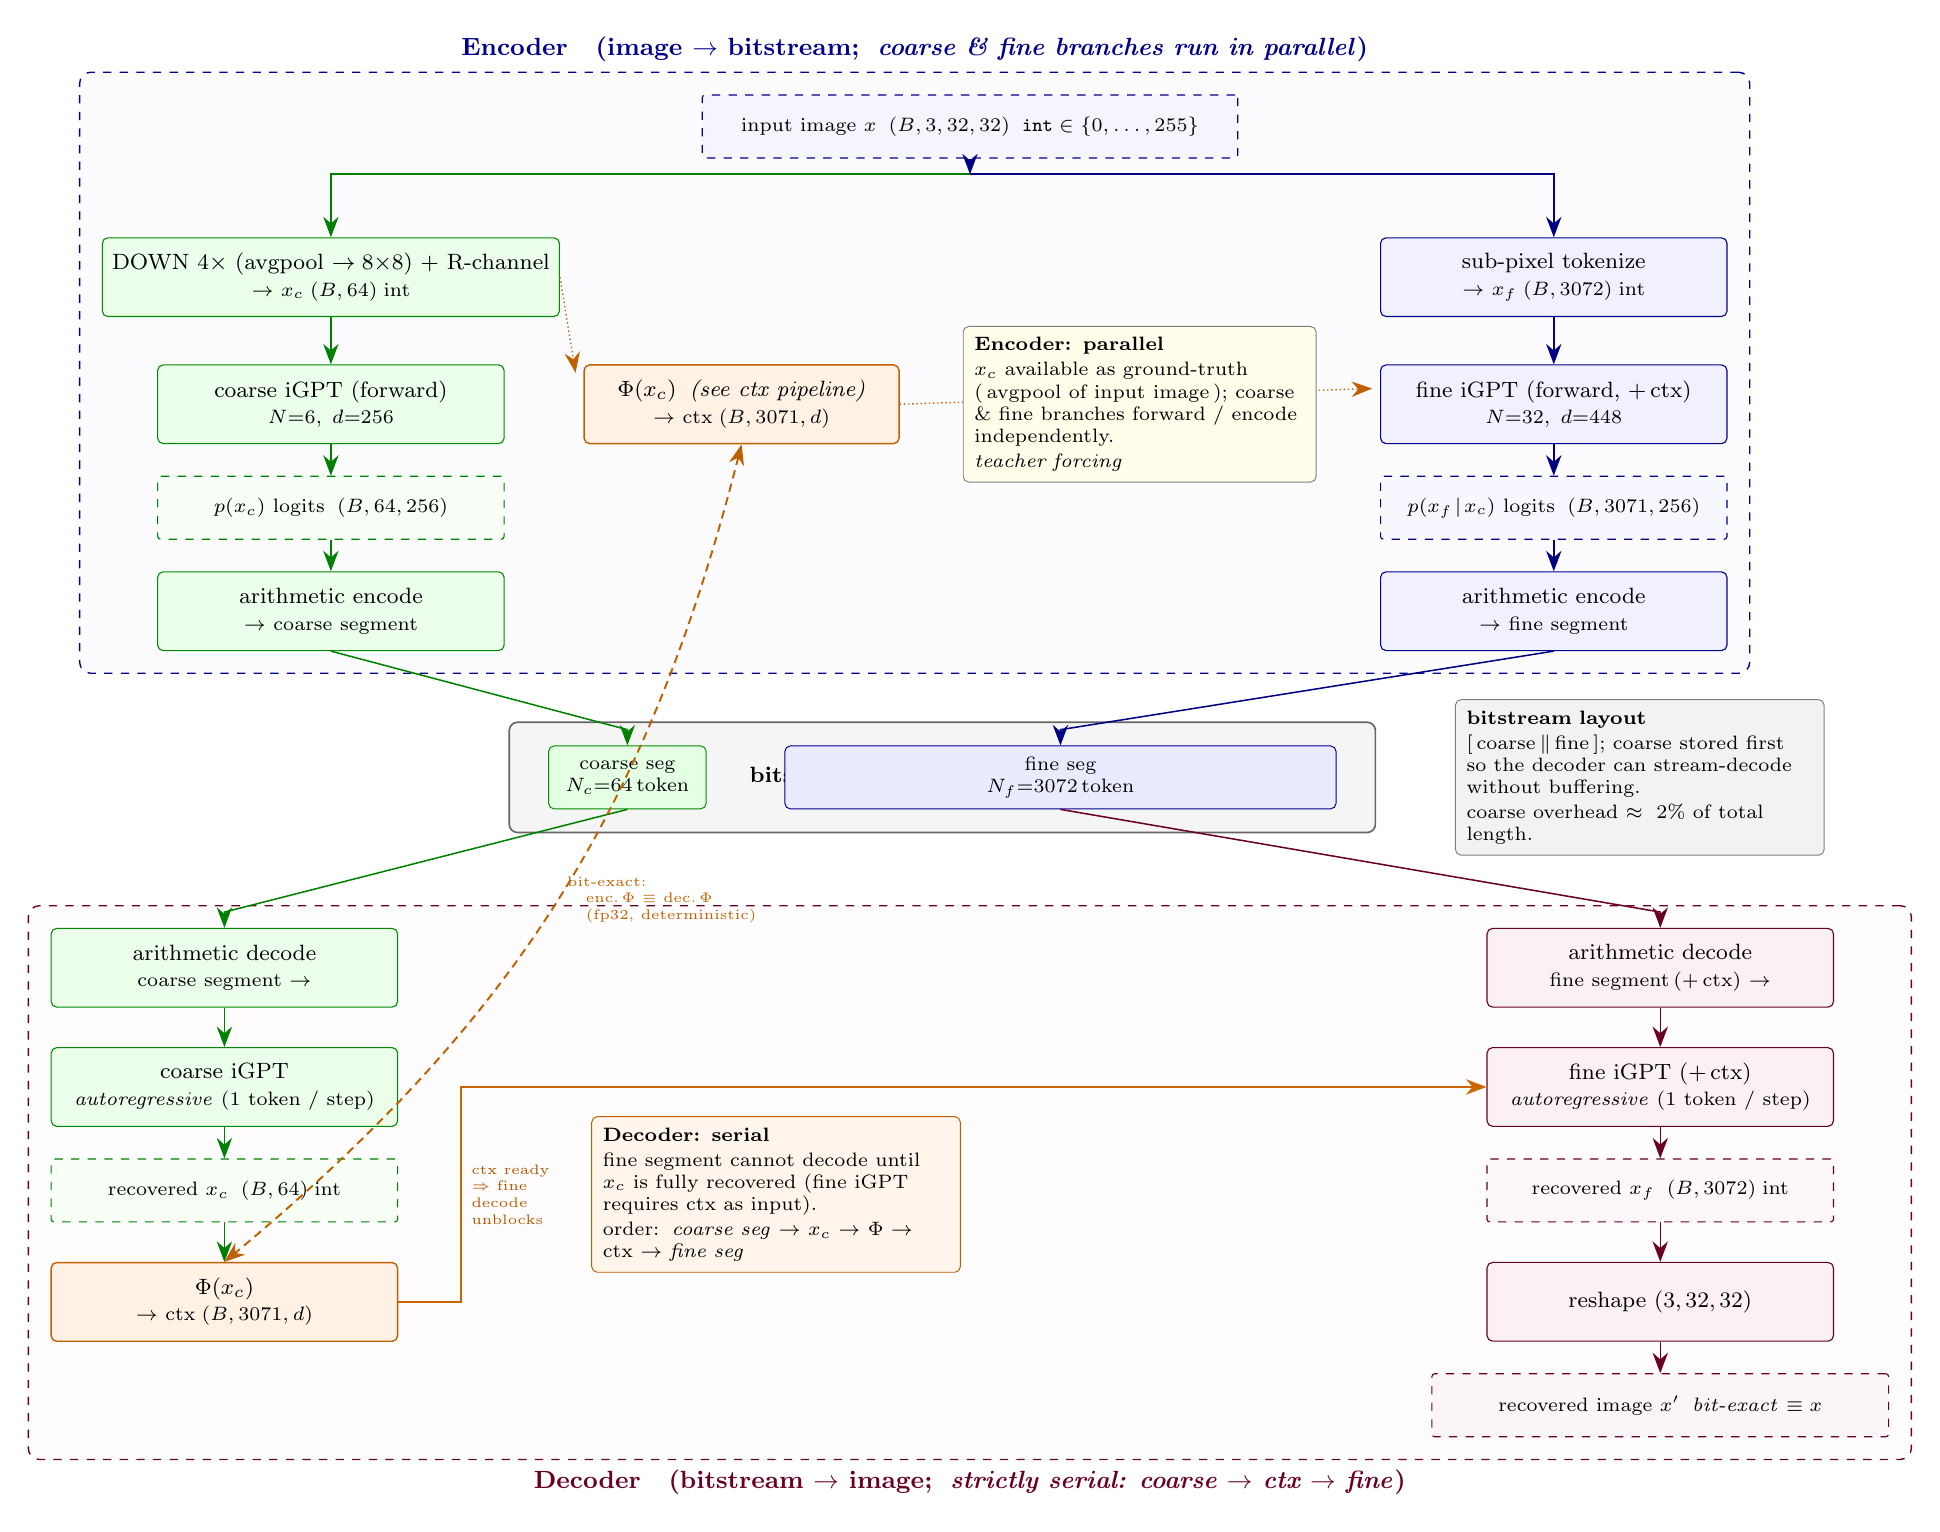
\begin{tikzpicture}[
    font=\footnotesize,
    >={Stealth[length=2.6mm]},
    node distance=8mm and 12mm,
    % ---- encoder-side blocks (top half, blue) ----
    encbox/.style ={draw, rounded corners=2pt, align=center,
                    minimum height=10mm, minimum width=44mm,
                    inner sep=3.5pt, fill=blue!6, draw=blue!55!black,
                    line width=0.4pt},
    % ---- decoder-side blocks (bottom half, purple) ----
    decbox/.style ={draw, rounded corners=2pt, align=center,
                    minimum height=10mm, minimum width=44mm,
                    inner sep=3.5pt, fill=purple!6, draw=purple!55!black,
                    line width=0.4pt},
    % ---- coarse-branch tint (green, both halves) ----
    coarsebox/.style={draw, rounded corners=2pt, align=center,
                      minimum height=10mm, minimum width=44mm,
                      inner sep=3.5pt, fill=green!8, draw=green!55!black,
                      line width=0.4pt},
    % ---- ctx box (orange, the bit-exact bridge) ----
    ctxbox/.style ={draw, rounded corners=2pt, align=center,
                    minimum height=10mm, minimum width=44mm,
                    inner sep=3.5pt, fill=orange!10, draw=orange!75!black,
                    line width=0.5pt},
    % ---- bitstream container (center, big) ----
    bsbox/.style  ={draw, rounded corners=3pt, align=center,
                    minimum height=14mm, minimum width=110mm,
                    inner sep=5pt, fill=gray!8, draw=black!60,
                    line width=0.6pt},
    bsseg/.style  ={draw, rounded corners=2pt, align=center,
                    minimum height=8mm, inner sep=3pt,
                    font=\scriptsize, line width=0.35pt},
    % ---- image / tensor pill ----
    imgpill/.style={draw, rounded corners=1pt, align=center,
                    fill=gray!4, draw=gray!55, font=\scriptsize,
                    inner sep=3pt, minimum width=44mm,
                    minimum height=8mm, dashed},
    % ---- arrows ----
    flow/.style    ={->, line width=0.55pt, blue!50!black},
    decflow/.style ={->, line width=0.55pt, purple!55!black},
    coflow/.style  ={->, line width=0.55pt, green!50!black},
    biteq/.style   ={<->, line width=0.7pt, orange!75!black, densely dashed},
    % ---- callout ----
    callout/.style ={draw=black!50, rounded corners=2pt,
                     fill=yellow!8, align=left, font=\scriptsize,
                     inner sep=4pt, line width=0.35pt},
]

% =========================================================
% TOP: encoder input (image x)
% =========================================================
\node[imgpill, fill=blue!4, draw=blue!55!black, minimum width=68mm]
     (xin) {input image $x$\;\;$(B,3,32,32)$\;\;\texttt{int}\;$\in\{0,\dots,255\}$};

% =========================================================
% Encoder split: x feeds BOTH branches in parallel
% =========================================================
% LEFT branch (coarse) and RIGHT branch (fine) at the same row
\node[coarsebox, below left=10mm and 18mm of xin]
     (e_avg) {DOWN $4{\times}$ (avgpool $\to 8{\times}8$) + R-channel\\\scriptsize $\to$ $x_c$\;$(B,64)$\;int};
\node[encbox, below right=10mm and 18mm of xin]
     (e_tok) {sub-pixel tokenize\\\scriptsize $\to$ $x_f$\;$(B,3072)$\;int};

% Coarse encoder chain
\node[coarsebox, below=6mm of e_avg] (e_cgpt)
     {coarse iGPT (forward)\\\scriptsize $N{=}6,\;d{=}256$};
\node[imgpill, below=4mm of e_cgpt, fill=green!3, draw=green!50!black]
     (e_cprob) {$p(x_c)$ logits\;\;$(B,64,256)$};
\node[coarsebox, below=4mm of e_cprob] (e_cac)
     {arithmetic encode\\\scriptsize $\to$ coarse segment};

% Fine encoder chain
\node[encbox, below=6mm of e_tok] (e_fgpt)
     {fine iGPT (forward, +\,ctx)\\\scriptsize $N{=}32,\;d{=}448$};
\node[imgpill, below=4mm of e_fgpt, fill=blue!3, draw=blue!50!black]
     (e_fprob) {$p(x_f\!\mid\! x_c)$ logits\;\;$(B,3071,256)$};
\node[encbox, below=4mm of e_fprob] (e_fac)
     {arithmetic encode\\\scriptsize $\to$ fine segment};

% Encoder-side ctx (between the two chains, fed to fine)
\node[ctxbox, right=10mm of e_cgpt, minimum width=40mm]
     (e_phi) {$\Phi(x_c)$\;\;\textit{(see ctx pipeline)}\\\scriptsize $\to$ ctx\;$(B,3071,d)$};

% =========================================================
% Center: bitstream box (the meeting point)
% =========================================================
\node[bsbox, below=14mm of $(e_cac)!0.5!(e_fac)$] (bs)
     {\textbf{bitstream} \;(persistent / wire / disk)};
\node[bsseg, fill=green!10, draw=green!55!black, minimum width=20mm]
     at ($(bs.center)+(-40mm,0)$)
     (bsCo) {coarse seg\\$N_c{=}64$\,token};
\node[bsseg, fill=blue!8, draw=blue!55!black, minimum width=70mm]
     at ($(bs.center)+(15mm,0)$)
     (bsFi) {fine seg\\$N_f{=}3072$\,token};

% =========================================================
% BOTTOM: decoder chain (strictly serial)
% =========================================================
% Decoder coarse branch (LEFT, mirrors encoder)
\node[coarsebox, below left=12mm and 14mm of bs] (d_cac)
     {arithmetic decode\\\scriptsize coarse segment $\to$};
\node[coarsebox, below=5mm of d_cac] (d_cgpt)
     {coarse iGPT\\\scriptsize \emph{autoregressive} (1 token / step)};
\node[imgpill, below=4mm of d_cgpt, fill=green!3, draw=green!50!black]
     (d_xc) {recovered $x_c$\;\;$(B,64)$\;int};
\node[ctxbox, below=5mm of d_xc, minimum width=44mm]
     (d_phi) {$\Phi(x_c)$\\\scriptsize $\to$ ctx\;$(B,3071,d)$};

% Decoder fine branch (RIGHT, depends on ctx)
\node[decbox, below right=12mm and 14mm of bs] (d_fac)
     {arithmetic decode\\\scriptsize fine segment\,(+\,ctx) $\to$};
\node[decbox, below=5mm of d_fac] (d_fgpt)
     {fine iGPT (+\,ctx)\\\scriptsize \emph{autoregressive} (1 token / step)};
\node[imgpill, below=4mm of d_fgpt, fill=purple!3, draw=purple!50!black]
     (d_xf) {recovered $x_f$\;\;$(B,3072)$\;int};
\node[decbox, below=5mm of d_xf] (d_reshape)
     {reshape $(3,32,32)$};
\node[imgpill, below=4mm of d_reshape, fill=purple!4, draw=purple!55!black,
      minimum width=58mm]
     (xout) {recovered image $x'$\;\;\textit{bit-exact} $\equiv x$};

% =========================================================
% Encoder arrows
% =========================================================
\draw[flow] (xin.south) -- ++(0,-2mm) coordinate (xsplit);
\draw[coflow] (xsplit) -| (e_avg.north);
\draw[flow]   (xsplit) -| (e_tok.north);

\draw[coflow] (e_avg) -- (e_cgpt);
\draw[coflow] (e_cgpt) -- (e_cprob);
\draw[coflow] (e_cprob) -- (e_cac);

\draw[flow] (e_tok) -- (e_fgpt);
\draw[flow] (e_fgpt) -- (e_fprob);
\draw[flow] (e_fprob) -- (e_fac);

% encoder ctx feed: x_c (avg/coarse output) -> Phi -> fine iGPT
\draw[->, line width=0.5pt, orange!75!black, densely dotted]
     (e_avg.east) -- ($(e_phi.west)+(-1mm,4mm)$);
\draw[->, line width=0.5pt, orange!75!black, densely dotted]
     (e_phi.east) -- ($(e_fgpt.west)+(-1mm,2mm)$)
     node[midway, above, font=\tiny, orange!60!black]
     {$\alpha\!\cdot\!$ctx};

% encoder -> bitstream
\draw[coflow] (e_cac.south) -- ($(bsCo.north)+(0,2mm)$) -- (bsCo.north);
\draw[flow]   (e_fac.south) -- ($(bsFi.north)+(0,2mm)$) -- (bsFi.north);

% =========================================================
% Decoder arrows
% =========================================================
% bitstream -> decoder
\draw[coflow] (bsCo.south) -- ($(d_cac.north)+(0,2mm)$) -- (d_cac.north);
\draw[decflow] (bsFi.south) -- ($(d_fac.north)+(0,2mm)$) -- (d_fac.north);

% decoder coarse chain
\draw[coflow] (d_cac) -- (d_cgpt);
\draw[coflow] (d_cgpt) -- (d_xc);
\draw[coflow] (d_xc) -- (d_phi);

% the critical cross-coupling: Phi -> fine decoder (serial dependency)
\draw[->, line width=0.7pt, orange!80!black]
     (d_phi.east) -- ++(8mm,0) |- (d_fgpt.west)
     node[pos=0.25, right, font=\tiny, orange!70!black, align=left,
          name=unblockLbl]
     {ctx ready\\$\Rightarrow$ fine\\decode\\unblocks};

% decoder fine chain
\draw[decflow] (d_fac) -- (d_fgpt);
\draw[decflow] (d_fgpt) -- (d_xf);
\draw[decflow] (d_xf) -- (d_reshape);
\draw[decflow] (d_reshape) -- (xout);

% =========================================================
% bit-exact equivalence (Phi enc == Phi dec) -- the central guarantee
% =========================================================
\draw[biteq] (e_phi.south) to[bend left=18]
             node[midway, right, font=\tiny, orange!75!black, align=left]
             {bit-exact:\\\quad enc.\,$\Phi$ $\equiv$ dec.\,$\Phi$\\\quad (fp32, deterministic)}
             (d_phi.north);

% =========================================================
% Section frames + labels
% =========================================================
\begin{pgfonlayer}{background}
  % Encoder frame (top half)
  \node[draw=blue!55!black, dashed, rounded corners=4pt,
        fill=blue!1, line width=0.5pt, inner sep=8pt,
        fit=(xin)(e_avg)(e_tok)(e_cgpt)(e_fgpt)(e_phi)(e_cac)(e_fac),
        label={[blue!55!black, font=\small\bfseries]above:%
              \textbf{Encoder} \; (image $\to$ bitstream;\;
              \emph{coarse \& fine branches run in parallel})}]
        (encframe) {};

  % Decoder frame (bottom half)
  \node[draw=purple!55!black, dashed, rounded corners=4pt,
        fill=purple!1, line width=0.5pt, inner sep=8pt,
        fit=(d_cac)(d_fac)(d_cgpt)(d_fgpt)(d_xc)(d_phi)(d_xf)(d_reshape)(xout),
        label={[purple!55!black, font=\small\bfseries]below:%
              \textbf{Decoder} \; (bitstream $\to$ image;\;
              \emph{strictly serial: coarse $\to$ ctx $\to$ fine})}]
        (decframe) {};
\end{pgfonlayer}

% =========================================================
% Right-side legend / callouts
% =========================================================
\node[callout, right=8mm of e_phi, text width=42mm, anchor=west]
     (legA) {\textbf{Encoder: parallel}\\[1pt]
             $x_c$ available as ground-truth (\,avgpool of input image\,);
             coarse \& fine branches forward / encode independently.\\[1pt]
             \textit{teacher forcing}};

\node[callout, right=4mm of unblockLbl, anchor=west, text width=44mm,
      fill=orange!8, draw=orange!75!black]
     (legB) {\textbf{Decoder: serial}\\[1pt]
             fine segment cannot decode until $x_c$ is fully recovered
             (fine iGPT requires ctx as input).\\[1pt]
             order:\;\;\emph{coarse seg} $\to$ $x_c$ $\to$ $\Phi$ $\to$ ctx
             $\to$ \emph{fine seg}};

\node[callout, right=10mm of bs, text width=44mm, anchor=west,
      fill=gray!10, draw=black!50]
     (legBS){\textbf{bitstream layout}\\[1pt]
             $[\,\text{coarse}\,\Vert\,\text{fine}\,]$;
             coarse stored first so the decoder can stream-decode
             without buffering.\\[1pt]
             coarse overhead $\approx 2\%$ of total length.};

\end{tikzpicture}
\end{document}
